%!TEX root = ../these.tex

\section{
  Визуализация геометрической информации
}
\label{ch:json.view}

Использование открытых форматов файлов позволило
также значительно упростить вопросы,
связанные с визуализацией обрабатываемой информации.
Традиционно для этого приходится
писать отдельный код,
имеющий зачастую довольно сложную структуру и решающий
множество задач, включая геометрические расчёты
и организацию пользовательского интерфейса.
В рамках данной диссертационной работы
в качестве средства визуализации
использовался экспорт в формат
Scalable Vector Graphics
(SVG),
который является стандартом де-факто,
содержит богатые возможности визуализации
и широко поддержан всеми современными браузерами.
Листинг~\ref{lst:json-svg}
показывает пример простейшего SVG-файла,
сгенерированного для раскройной карты,
представленной на Листинге~\ref{lst:json-dbs}.

\lstinputlisting[
  language=XML,
  basicstyle=\footnotesize,
  showstringspaces=false,
  numbers=left,
  label={lst:json-svg},
  captionpos=b,
  caption=SVG-файл для визуализации раскроя из Листинга~\ref{lst:json-dbs}
  ]
  {media/nesting.svg}

Переход к широкому использованию SVG
позволяет также использовать зрелые современные технологии
каскадных таблиц стилей
(Cascading Style Sheets, CSS)
для управления внешним видом визуализации
(включая цвета, заливки и штриховки и анимацию)
и язык JavaScript
для добавления к визуализации
элементов интерактивности.
Один из вариантов оформления
SVG-файла из Листинга~\ref{lst:json-svg}
приведён на рис.~\ref{fig:json-nesting}.
Пользовательский интерфейс
(масштабирование и прокрутка)
обеспечивается при помощи подключения
библиотеки с открытым кодом
svg-pan-zoom~\cite{bi:svg-pan-zoom}.

\begin{figure}
  \centering
  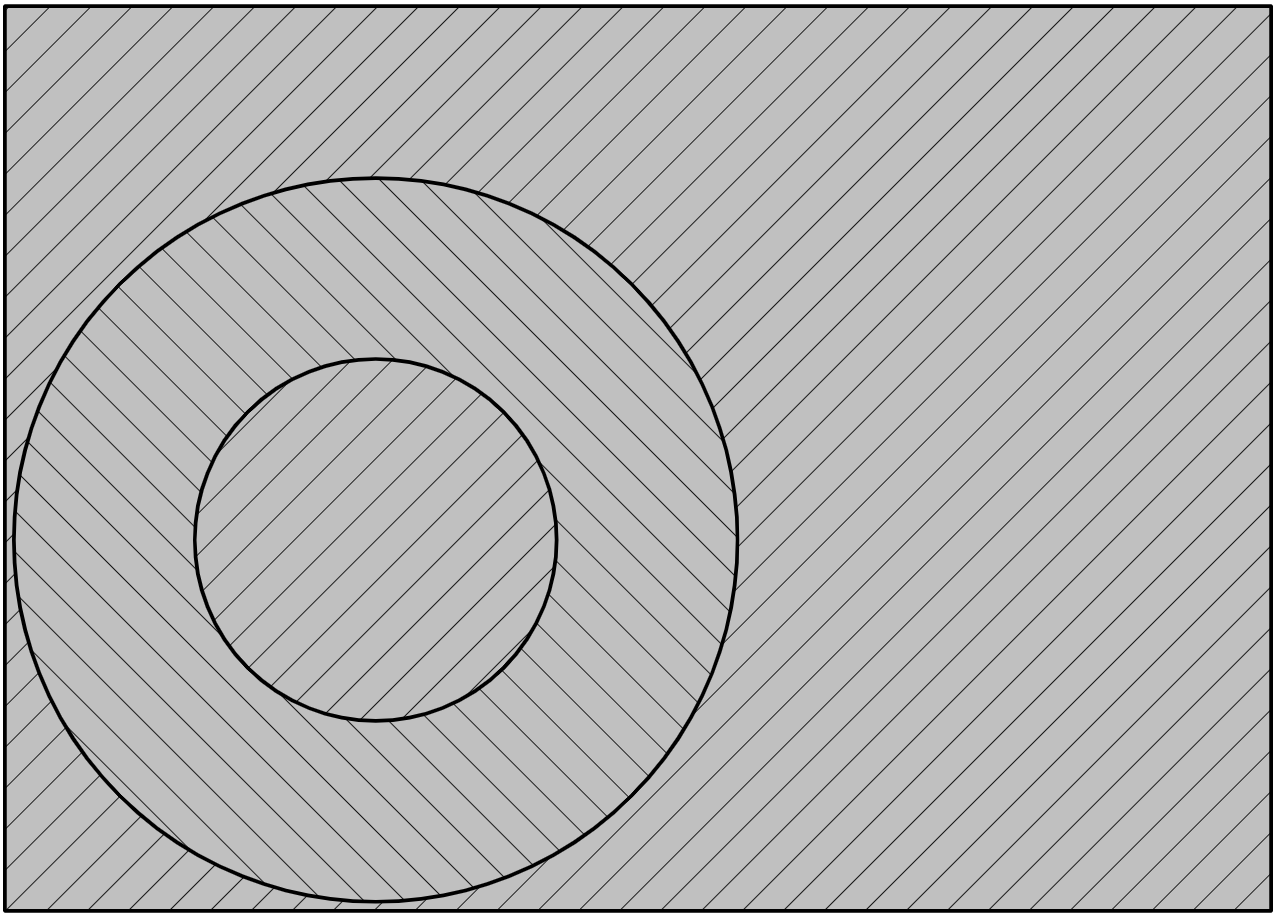
\includegraphics[width=0.5\textwidth]{nesting.png}
  \caption{Визуализация раскроя из Листинга~\ref{lst:json-dbs}}
  \label{fig:json-nesting}
\end{figure}

В ходе диссертационной работы
была разработан пакет утилит
\cite{bi:dbs2json},
обеспечивающих конвертацию между
различными форматами файлов
(включая DBS, JSON, YAML, DXF и SVG для визуализации).
Для визуализации решения задачи PCGTSP
(на основе комбинации информации,
полученной из нескольких источников),
была разработана специализированная утилита
\cite{bi:j2pcgtsp},
первоначально в форме утилиты командной строки
но позднее преобразованная
для удобства использования в
Single Page Application
(SPA).
Пример созданного ею изображения
приведён на рис.~\ref{fig:pcgtsp.svg},
стр.~\pageref{fig:pcgtsp.svg}.
